\documentclass[a4paper, 10pt, superscriptaddress, nofootinbib, showkeys, notitlepage]{revtex4-1}
%!TEX encoding = UTF-8 Unicode
%%%%%%%%%%%%%%%%%%%%
\usepackage[english]{babel}
\usepackage{amsmath, amssymb, amsfonts, amscd, amsthm}
\usepackage[a4paper,top=3.5cm,bottom=3cm,left=2.5cm,right=2.5cm,bindingoffset=5mm]{geometry}
\usepackage{dsfont}
\usepackage{mathrsfs}
\usepackage{stmaryrd}
\usepackage[utf8x]{inputenc}
\usepackage{indentfirst}
\usepackage{microtype}
\usepackage[margin=1.5cm, labelfont=it]{caption}
\usepackage{textcomp}
\usepackage{graphicx}%insert figures
\usepackage{float}
\usepackage{array, booktabs}
\usepackage[colorlinks=true, linkcolor = blue, citecolor= red, urlcolor= red]{hyperref}
\usepackage{tikz, tikz-cd}
\usetikzlibrary{arrows, calc, shapes, fit, matrix, decorations.pathreplacing, decorations.markings, decorations.pathmorphing, positioning, fadings, patterns, chains}
\usepackage[all]{xy}
\usepackage{stackengine,scalerel}
\usepackage{mathtools}
\usepackage{cleveref}

%%%%%%%%%%%%%%%%%%%%%%%%%%%%%%%%%

%%%%%%Command redefinitions%%%%%%%

%%%%%%%%%%%%%%%%%%%%%%%%%%%%%%%%%

%%%%%%%%%%%%%%%%%%%%%Abstract environment definition%%%%%%%%%%%%%%%%
%\renewenvironment{abstract}{\begin{center}\begin{minipage}{0.77\textwidth}\rule{\textwidth}{0.04em}\\[0.4em]\small\textbf{\abstractname~|}}{\par\rule{\textwidth}{0.04em}\end{minipage}\end{center}}
%%%%%%%%%%%%%%%%%%%%%%%%%%%%%%%%%%%%%%%%%%%%%%%%%%%%

%
%%
%%%
%%%%%%
%%%%%%%%%
%%%%%%%%%%%%
%%%%%%%%%
%%%%%%
%%%
%%
%
\begin{document}

%%%%%%Authors details%%%%%%

\author{Oscar de Felice}
%%
	\affiliation{via dei Genovesi 92, 09124 Cagliari, Italy}
%%
	{\let\thefootnote\relax\footnote{\hspace{-4ex}\textsuperscript{1}\emph{e-mail}: \href{mailto:oscar.defelice@gmail.com}{oscar.defelice@gmail.com}}}
%%%
\author{Gustavo de Felice}
%%
	\affiliation{via Silvio Pellico 12, 84073 Sapri, Italy}
%%
	{\let\thefootnote\relax\footnote{\hspace{-4ex}\textsuperscript{2}\emph{e-mail}: \href{mailto:gustavo@dottordefelice.it}{gustavo@dottordefelice.it}}}
%%%


%%%%
%%%%%%%%%%%%%%%%%%%%

\date{\today}
%
%%
%%%
%%
%
%
%%%%%%Title%%%%%%%%%%%%
\title{A supervised image recognition approach to diagnose dental diseases}
%%%%%%%%%%%%%%%%%%%%
%
%%%%%%%%%%%%
\begin{abstract}
%
	The main goal of this document is to describe the idea of image recognition to determine whether a patient may have some odontoiatric disease.
	Briefly, we aim to use a machine learning approach, training an image recognition algorithm over an image database, labelled with the diseases and use the fitted model to predict whether a new image has the features characterising a specific illness. The idea is to give suggestions to doctors alerting them when an image is found with an high probability of a disease.
	The approach is general, however 
%
\end{abstract}
%%%%%%%%%%%%%
%
\maketitle
%
%%

\section*{Introduction}
	%
	An important issue to face since the birth of image recognition techniques is the detection and classification of objects in digital images. 
	Obviously, objects can be classified by several aspects, \emph{e.g.} colours, textures, shapes, position within images, etc.
	
	Recently, there have been several satisfying examples of the use of such approach~\cite{stocazzo1}. 
	Even back to the early 2000's, one can find contributions to the applications image recognition to medical diagnostic systems~\cite{stocazzo2}.
	%
	
	%%%%%
	%%%
	%%
	%
\section{A warm-up example: facial recognition}
	%
	Just to illustrate the method, we want to describe a simple image recognition algorithm. 
	The basic idea is to detect faces in pictures.
	This is a typical example of supervised learning algorithm, largely used in social networks. 
	%
	
	%%%
	%%
	%
\subsection{Understanding how face recognition works}
	%
	
		%
		\begin{figure}
  			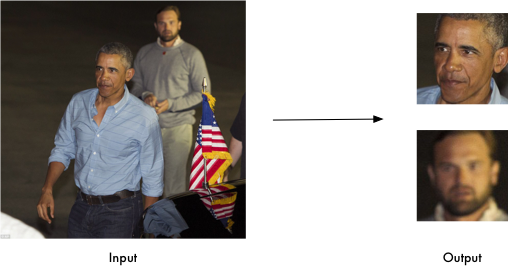
\includegraphics[width=.7\linewidth]{Images/Obama.png}
 			\caption{Working scheme of the face recognition algorithm.}
 			\label{fig:obama}
		\end{figure}
		%
	%
	
	%%%%%
	%%%
	%%
	%
\section{Overview of diagnostic systems based on automatic image recognition}
	%
	In this section we review the general scheme of diagnostic systems based on a machine learning approach. 
	In particular, we are going to expose the working mechanism of image recognition algorithms applied to medical diagnosis.
	
	%
	
	%%%
	%%
	%
\subsection{Shape characterisation}
	%
	Mathematically, images can be thought as sets of connected points in a two-dimensional space $\mathcal{F}$, often (and also here) approximated in a discrete binary space.
	People do not perform image classification directly on $\mathcal{F}$, since this task is computationally really expensive ($\sim \mathcal{O}(n^2)$), where each image is made up by $n$ pixels.
	The representation of an image can be modified by an image transformation, by mapping the space $\mathcal{F}$ to a -- typically smaller -- feature space $\mathcal{F}'$.
	
	%
	
	%%%
	%%
	%
\subsection{Gauged Supergravity}
	%

	%
	
	%%
	%
\subsubsection*{Isometries}
	%

	%

	%%
	%
\subsubsection*{Magnetic gaugings}
	%
	
	%	
	%%%%%
	%%%
	%%
	%
\section{Things to know}
	%
	
	%

	%%%
	%%
	%
\subsection{\texorpdfstring{Attractor mechanism for $\mathrm{AdS}$ black holes}{Attractor mechanism for AdS black holes}}
	%
	
	%	
	
	%%%
	%%
	%
\subsection{The topologically twisted index}
	%
	
	%
	%%%%
	%%%
	%%
	%
\subsubsection*{\texorpdfstring{The topologically twisted index at large $N$}{The topologically twisted index at large N}}
	%

	%
	%%%
	%%
	%
\subsection{\texorpdfstring{Dyonic $ISO(7)$ supergravity}{Dyonic ISO(7) supergravity}}
	%
	
	%	
	%%%
	%%
	%
	%%%%%%%%%%%%%%%%%%%%%%%%%%%%%%%%%%%%%%%%%%%%%%%%%%%%%%%%%%%%%%%%%%%%%%%%%%%%%%%%
%%%%%%%%%%%%%%%%%%%%%%%%%%%%%%%%%%%%%%%%Appendices%%%%%%%%%%%%%%%%%%%%%%%%%%%%%%%%%%%%%%%%
	%%%%%%%%%%%%%%%%%%%%%%%%%%%%%%%%%%%%%%%%%%%%%%%%%%%%%%%%%%%%%%%%%%%%%%%%%%%%%%%%
	%
	%%
	%%%
	%%%%
	%%%
	%%
	%
	\appendix
	%
	%%
	%%%
	%%%%
	%%%
	%%
	%
\section{\texorpdfstring{Reduction from $E_{7(7)}$}{Reduction from E7(7)}}
	%
	
	%
	%%%
	%%
	%
	%Appendix 
	%%%%
	%%%
	%%
	%
\section{Reduction to the \texorpdfstring{$SU(2)$}{SU(2)}-invariant sector}
	%	
	
	%	
	%%%
	%%
	%
	%%%%%%%%%%%%%%Appendices%%%%%%%%%%%%%%%%%%%
	%
	%%
	%%%
%
	%%%
% 	%%
% 	%
% 	%
% 	
%%%%%Bibliography%%%%
\bibliographystyle{unsrtsiam2}
\bibliography{Bibliography}
\nocite{*}
%%%%%%%%%%%%%%%

\end{document}
